\begin{frame}
	\vspace{2cm}
	\begin{center}
		{\Huge\textbf{\textcolor{copenhagenred}{Unbiased MCMC}}}
		\vspace{1cm}

		\rule{4cm}{3pt}
		\vspace{2cm}
	\end{center}
\end{frame}

\begin{frame}{The Problem with Traditional MCMC}
	\begin{columns}
		\column{0.5\textwidth}
		\textbf{Traditional MCMC Challenges:}
		\begin{itemize}
			\item \alert{Burn-in bias}: Initial samples don't follow target distribution
			\item \alert{Convergence diagnostics}: When to stop burn-in?
			\item \alert{Multiple chains}: same issues as above and the bias prevents the consistent estimation
			      of by averages over the independent runs.
		\end{itemize}

		\vspace{0.5cm}
		\textbf{Consequence:}\\
		Must discard unknown number of initial samples, limiting parallel efficiency

		\column{0.5\textwidth}
		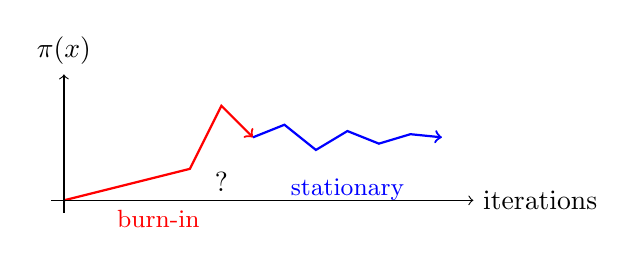
\begin{tikzpicture}[scale=0.8]
			% Draw burn-in phase
			\draw[thick,red,->] (0,0) -- (2,0.5) -- (2.5,1.5) -- (3,1);
			\node[red,below] at (1.5,0) {\small burn-in};

			% Draw stationary phase
			\draw[thick,blue,->] (3,1) -- (3.5,1.2) -- (4,0.8) -- (4.5,1.1) -- (5,0.9) -- (5.5,1.05) -- (6,1);
			\node[blue,below] at (4.5,0.5) {\small stationary};

			% Axes
			\draw[->] (-0.2,0) -- (6.5,0) node[right] {iterations};
			\draw[->] (0,-0.2) -- (0,2) node[above] {$\pi(x)$};

			% Question mark
			\node at (2.5,0.3) {?};
		\end{tikzpicture}

	\end{columns}
\end{frame}

\begin{frame}{The Unbiased MCMC Solution}
	\begin{block}{Key Innovation: Coupling + Debiasing}
		Run two coupled Markov chains that eventually meet, then use their difference to construct an \alert{unbiased estimator}
	\end{block}

	\vspace{0.5cm}
	\begin{columns}
		\column{0.45\textwidth}
		\textbf{The Algorithm:}
		\begin{enumerate}
			\item Start chains $X_1$ and $Y_0$ from initial distribution
			\item Run coupled chains until meeting time $\tau = \inf\{t \geq 1 : X_t = Y_{t-1}\}$
			\item Compute debiased estimator:
		\end{enumerate}

		\column{0.45\textwidth}
		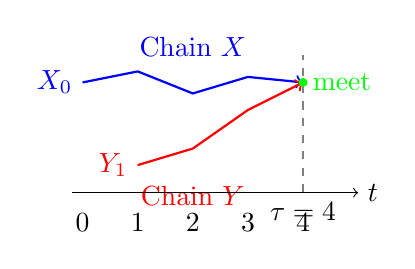
\begin{tikzpicture}[scale=0.7]
			% Chain X
			\draw[thick,blue,->] (0,2) node[left] {$X_0$} -- (1,2.2) -- (2,1.8) -- (3,2.1) -- (4,2);
			\node[blue,above] at (2,2.3) {Chain $X$};

			% Chain Y
			\draw[thick,red,->] (1,0.5) node[left] {$Y_1$} -- (2,0.8) -- (3,1.5) -- (4,2);
			\node[red,below] at (2,0.3) {Chain $Y$};

			% Meeting point
			\draw[dashed,gray] (4,0) -- (4,2.5);
			\node[below] at (4,0) {$\tau=4$};
			\filldraw[green] (4,2) circle (2pt);
			\node[green,right] at (4,2) {meet};

			% Time axis
			\draw[->] (-0.2,0) -- (5,0) node[right] {$t$};
			\foreach \x in {0,1,2,3,4}
			\node[below] at (\x,-0.2) {\x};
		\end{tikzpicture}
	\end{columns}
\end{frame}

\begin{frame}{Glynn--Rhee Estimator}
	Given a target function $h$, two initial values
	$X_{0}\sim \pi_{0}$, $Y_{0}\sim \pi_{0}$, and
	$X_{1}\sim K(X_0,\cdot)$
	and set the coupled kernel as $$(X_{t+1},Y_{t})\sim \bar{K}((X_{t},Y_{t-1}),(\cdot,\cdot)), \quad \forall t\geq1$$
	with marginals equal to $K$ and meeting time $\tau$ as defined above.

	Under the assumptions:
	\begin{enumerate}
		\item  $E_\pi[h(X)] = \lim_{t \to \infty} E[h(X_t)]$ for $t\rightarrow \infty$
		\item meeting time decrease at geometric rate, i.e. $P(\tau >t)\leq C\delta^{t}$
		\item and that the chains stay together after they met, i.e. $X_t = Y_{t-1} \quad \forall t \geq \tau$
	\end{enumerate}

	Then for any fixed $k \ge 0$ the \textbf{Glynn--Rhee estimator}:

	$$H = h(X_k) + \sum_{t = k+1}^{\tau-1} [h(X_t) - h(Y_{t-1})]$$
	has expectation $E_{\pi}[h(X)].$
\end{frame}

\begin{frame}
	\frametitle{Glynn--Rhee proof sketch}
	\begin{itemize}
		% \item \textbf{Assumption 1}: To ensure existence of moments
		\item \textbf{Assumption 2}: This is the hardest to verify in practice. It requires the coupling to be efficient enough so that the meeting time has geometric tails
		\item \textbf{Assumption 3}: This is often easy to ensure in practice by designing the coupling appropriately
	\end{itemize}

	\begin{align*}
		 & E_\pi[h(X)] \underset{\text{by A1}}{=} \lim_{t \to \infty} E[h(X_t)] = E[h(X_k)] + \sum_{t=k+1}^{\infty} \{E[h(X_t)] - E[h(X_{t-1})]\} \\
		 & \underset{\text{by A2}}{=} E\left[h(X_k) + \sum_{t=k+1}^{\infty} [h(X_t) - h(\textcolor{red}{Y_{t-1}})]\right]
		\underset{\text{by A3}}{=} E\left[h(X_k) + \sum_{t=k+1}^{\textcolor{red}{\tau-1}} [h(X_t) - h(Y_{t-1})]\right]
	\end{align*}
	{\tiny we can replace $X_{t-1}$ by $Y_{t-1}$ since they have the marginal distribution
	and swap expectation and summation due to Fubini's theorem and Assumption 2 that ensure fast Convergence of the sum.
	\textbf{ESE=ES}}
\end{frame}

\begin{frame}
	\frametitle{Maximal Coupling of two Gaussians}
	\begin{figure}[h]
		\centering
		\includegraphics[width=0.4\textwidth]{maximal_coupling_plot.pdf}
		\caption{Maximal coupling of $\mathcal{N}(0, 1)$ and $\mathcal{N}(1, 1)$. Geometric interpretation: Maximizes mass on the diagonal.}
	\end{figure}
\end{frame}

\begin{frame}{Takeaways}
	\begin{itemize}
		\item No burn-in period required
		\item Since the estimator is unbiased, we can generate shorter chains (in parallel) and average them to reduce variance without introducing bias.
		\item However, the variance can be prohibitively high. Can be reduced by introducing lag $L$ and average $l$ iterations.
		\item The cost is more complexity in both execution and implementation and the need to design effective coupling strategies.
	\end{itemize}
\end{frame}
